\section{Methodology}

\subsection{Overview}
\noindent\hspace*{\parindent} Describe your overall approach or system design here.

\subsection{Example: Equation}
\noindent\hspace*{\parindent} Mathematical formulations use standard \texttt{amsmath} / \texttt{unicode-math} syntax, for example a state-space model:

\begin{equation}
    \dot{x}(t) = f\big(x(t), u(t)\big)
    \label{eq:example-dynamics}
\end{equation}

\noindent\hspace*{\parindent} where $x$ is the state vector and $u$ is the control input vector.

\subsection{Example: Figure}
\noindent\hspace*{\parindent} Figures are numbered per section (e.g. Figure~1.1 in Section~1) and listed in the List of Figures automatically.

\begin{figure}[H]
    \centering
    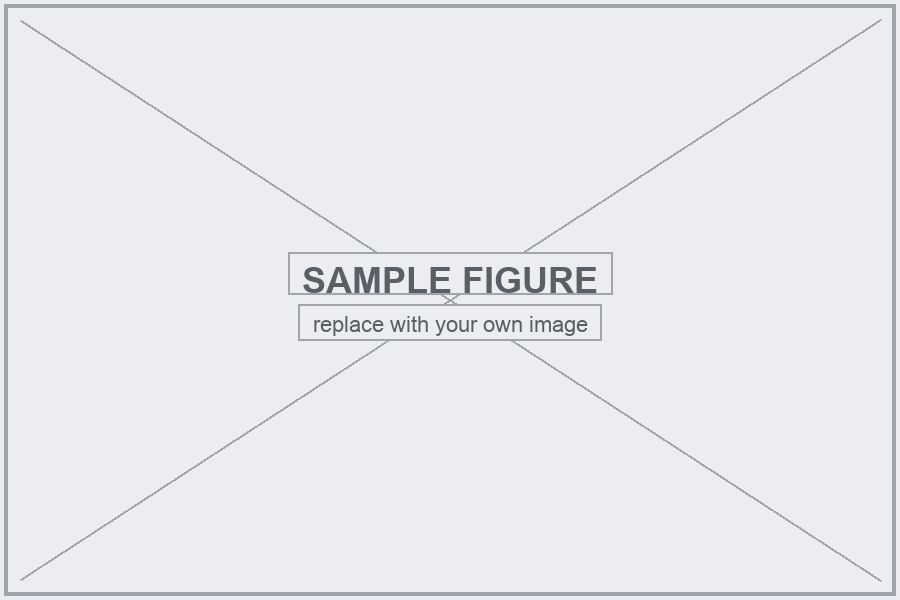
\includegraphics[width=0.6\textwidth]{figure/sample-figure.png}
    \caption{Example figure -- replace with your own diagram or plot}
    \label{fig:methodology-example}
\end{figure}

\subsection{Example: Table}
\noindent\hspace*{\parindent} Tables follow the same numbering convention as figures.

\begin{table}[H]
    \centering
    \caption{Example parameter table}
    \begin{tabular}{|l|c|}
    \hline
    \textbf{Parameter} & \textbf{Value} \\
    \hline
    Example parameter A & $1.0$ \\
    \hline
    Example parameter B & $0.5$ \\
    \hline
    \end{tabular}
    \label{table:example-params}
\end{table}

\subsection{Example: Algorithm}
\noindent\hspace*{\parindent} Pseudocode uses the \texttt{algorithm}/\texttt{algpseudocode} packages.

\begin{algorithm}[H]
    \caption{Example Algorithm}
    \begin{algorithmic}[1]
        \State Initialize variables
        \For{$i \gets 1$ \textbf{to} $N$}
            \State Perform an update step
        \EndFor
        \State \textbf{return} result
    \end{algorithmic}
\end{algorithm}

\subsection{Example: Code Block}
\noindent\hspace*{\parindent} Python code blocks use the custom \texttt{pythoncode} environment (syntax highlighting via \texttt{minted}).

\begin{pythoncode}
def example_function(x, u):
    """Replace with your own code example."""
    return x + u
\end{pythoncode}
